%==============================================================================
\chapter{Introduction}\label{cha:chapter1}
%==============================================================================
%
%
%
\begin{remark}{Outline}
    In this chapter, we present the heart and how it functions, from single cell excitation through to whole-organ contraction and relaxation (Section~\ref{sec:ch1physiology_of_the_heart}). We then present how the key physiological mechanisms at different biological scales can be modelled using equations of bio-electro-mechanics (Section~\ref{sec:ch1mathematical_modelling_of_the_heart}). Heart failure pathology is then introduced, with emphasis on the two most common phenotypes of the disease, namely when the ejection fraction is reduce and when it is preserved (Section~\ref{sec:ch1heart_failure}). We continue by stating the motivation for the research carried out within this thesis (Section~\ref{sec:ch1motivation_and_goals}), and we conclude with a brief summary (Section~\ref{sec:ch1summary}).
\end{remark}


%
%
%
\section{Physiology of the heart}\label{sec:ch1physiology_of_the_heart}
During each heartbeat, the chambers of the heart are activated by an electrical impulse that propagates across the entire tissue. The activation wave is initiated by a group of pacemaking cells, making up the \textit{sino-atrial} (\acs{SA}) \textit{node} and located in the right atrium, and immediately starts activating the atria before reaching the \textit{atrio-ventricular} (\acs{AV}) \textit{node}. The AV node slows down the activation signal before it passes to the \textit{atrio-ventricular bundle}. This allows the atria to fully contract to fill the ventricles with blood before the latters are activated. The activation signal through the AV bundle (which branches in two) spreads throughout the ventricles via the specialised, fast \textit{His-Purkinje} conduction system. The arrival of the activation wave at each cardiac muscle cell causes a depolarisation of the cell membrane that initiates an \textit{action potential} (\acs{AP}). This cellular electrical signal gives rise to a calcium transient that activates the tension generating proteins inside the cell through a process called \textit{excitation-contraction} (\acs{EC}) coupling. This causes the heart walls to contract, pumping blood in and out of the heart and around the body and to the lungs.

\begin{figure}[!ht]
    \myfloatalign
    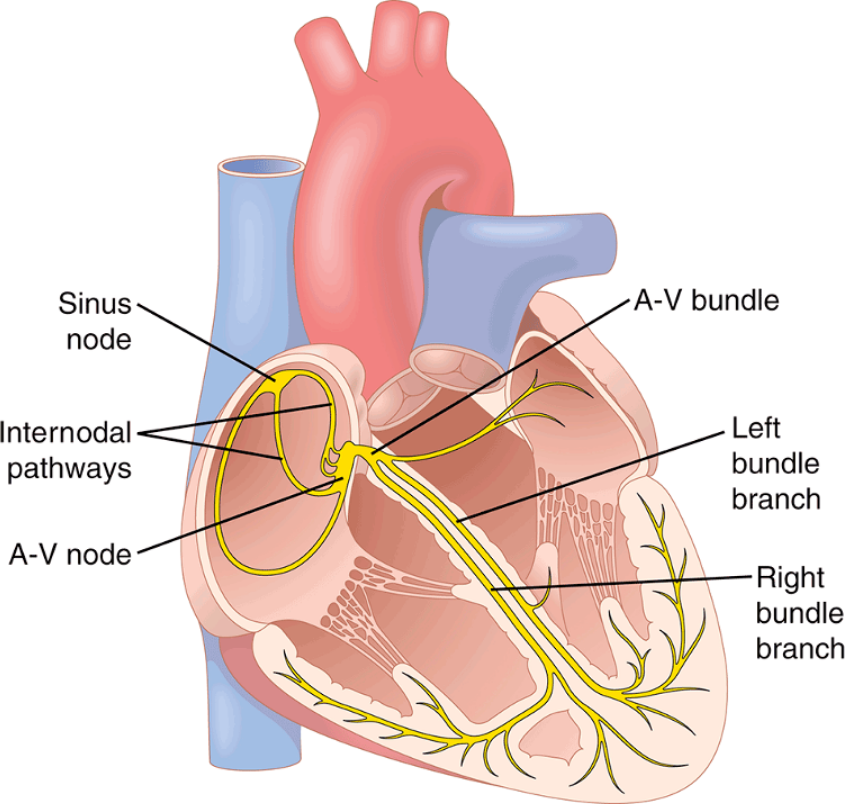
\includegraphics[width=0.66\textwidth]{figures/chapter01/fig_elsv_8.png}
    \caption{The heart and its conduction system. Adapted from~\cite{Guyton:2021}, Unit III, Chapter 10, Page 128, Figure 10-1. Copyright $\textcopyright$ 2021 by Elsevier, Inc.}
    \label{fig:heartcondactionsystem}
\end{figure}


%
%
%
\subsection{Cardiac electrophysiology}\label{sec:ch1cardiac_electrophysiology}
The surface membrane of a cardiac cell is called the \textit{sarcolemma}. On either side of the sarcolemma, the intracellular and the extracellular environments consist of ionic solutions. For cardiac electrophysiology the major ion species are sodium (\acs{Na}), potassium (\acs{K}), chloride (\acs{Cl}) and calcium (\acs{Ca}). An important property of the sarcolemma is its ability to maintain concentration gradients, such that each ion species is unevenly distributed between the intracellular and extracellular space, resulting in concentration gradients across the membrane. As ions are charged particles, their uneven distribution across the sarcolemma also creates an electrical gradient. The resulting electrochemical gradient provides a driving force to move ions across the cell membrane.

% (The diffusion gradient is also important so the voltage is not the sole force moving ions)

\vspace{0.2cm}
Another crucial property of the sarcolemma is its capacity to respond to electrical stimulation through the brief dynamic opening and closing of highly specific ion channels and electrogenic transporters to produce changes in its transmembrane potential. With each heartbeat, the cell membrane is depolarised and an AP is initiated as a result of a complex interplay of multiple ion channels, exchangers and transporters in the myocardium. A typical AP consists of five phases, each one associated with the opening of specific sarcolemma ion channels. The main ionic events at each AP phase can be summarised as follows.

\begin{description}
	\item[\textsc{Phase $0$.}] The initial depolarisation is due to opening of voltage-gated fast $\Na$ channels ($I_{Na}$) when the transmembrane voltage reaches the activation threshold of the channel between $\SI{-70}{}$ and $\SI{-60}{\milli\volt}$. Positive charged $\Na$ current flows rapidly into the cell due to the large $\Na$ concentration gradient and the negative transmembrane potential, leading to further depolarisation.
	\item[\textsc{Phase $1$.}] The early repolarisation of the AP is primarily caused by the rapidly activating and inactivating transient outward $\K$ current ($I_{to}$).
	\item[\textsc{Phase $2$.}] A plateau phase follows, resulting from a prolonged influx of $\Ca$ ions, as the voltage-gated L-type $\Ca$ channels ($I_{CaL}$) open upon depolarisation. This flow of $\Ca$ ions plays a crucial role in cardiac EC coupling, as it initiates a series of intracellular events that ultimately lead to myocardial contraction. Another current that contributes to the late Phase 2 plateau is the net inward current through the $\Na$/$\Ca$ \textit{exchanger} (\acs{NCX}) in $\Ca$ extrusion mode. This exchanger is a reversible counter-transport system that, when in forward ($\Ca$ extrusion) mode, uses the energy provided by the inward flux of $\Na$ ions down their electrochemical gradient to extrude $\Ca$ ions with a generally accepted stoichiometry of $3\colon 1$, thus moving one net charge into the cell. These two inward currents that determine the AP plateau are balanced by a reduced outward $\K$ current consequent to the membrane $\K$ conductance falling upon depolarisation. This phenomenon is called \textit{inward rectification}, caused by the obstruction of the inner mouth of $\K$ channels.
	\item[\textsc{Phase $3$.}] The outward flow of $\K$ ions is the major factor causing repolarisation that determines the duration of the AP. The large number of $\K$ channels can be divided into two molecular families: the voltage-gated channels and the inward rectifier channels. The voltage-gated outward $\K$ channels are the rapidly ($I_{Kr}$) and slowly ($I_{Ks}$) activating delayed rectifiers, and are responsible for repolarisation, fully activated at around $\SI{-10}{\milli\volt}$ and deactivated by full repolarisation. The inward rectifier $\K$ channels, such as the time-independent $\K$ current $I_{K1}$, help regulating the resting membrane potential and contribute to late Phase $3$ repolarisation.
	\item[\textsc{Phase $4$.}] $I_{K1}$ closes upon depolarisation and reopens during repolarisation to help terminate the AP and reset the membrane potential to the resting state, which for non-pacemaker cardiac cells such as the ventricular myocytes is around $\SI{-90}{mV}$. An important contribution to maintain resting membrane potential ionic homeostasis is given by the $\Na$/$\K$ \textit{ATPase} (\acs{NAK}). This is a key transporter and uses energy (in the form of \textit{adenosine triphosphate} (\acs{ATP})) to establish a low intracellular $\Na$ concentration and a high intracellular $\K$ concentration by moving $3$ $\Na$ ions out and $2$ $\K$ ions into the cell by hydrolisation of $1$ ATP molecule. This transport is \textit{electrogenic}, meaning that it results in the extrusion of $1$ net charge per cycle.
\end{description}

\begin{figure}[!ht]
    \myfloatalign
    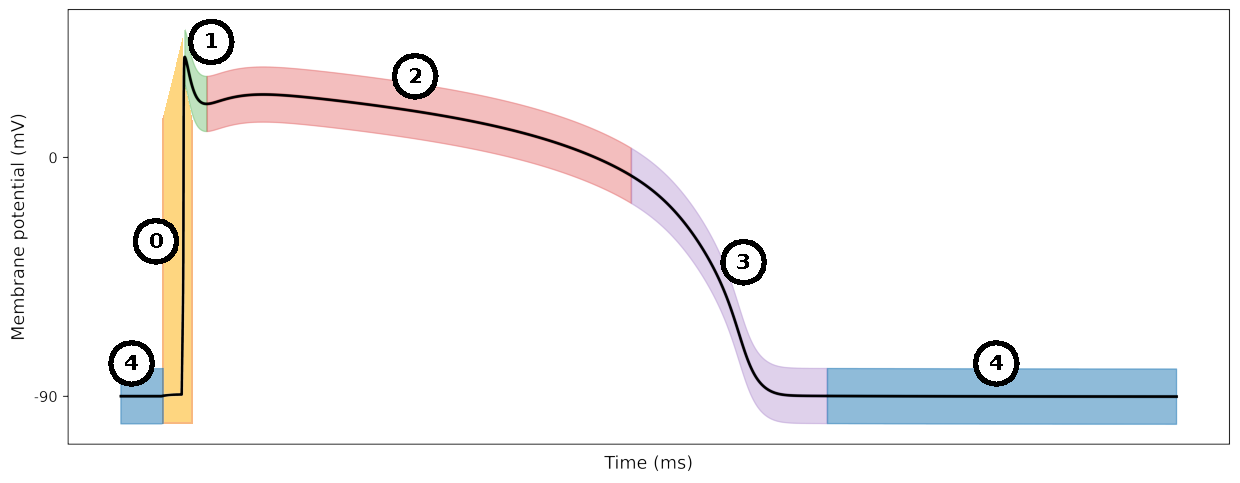
\includegraphics[width=\textwidth]{figures/chapter01/AP_phases.pdf}
    \caption{The five phases of an action potential in left ventricular myocytes.}
    \label{fig:my_label}
\end{figure}

\vspace{0.2cm}
Every ventricular myocyte is in general not excitable (\textit{refractory}) between Phase $0$ through to half way through Phase $3$, meaning that the cell cannot produce another AP. This is due to all the $\Na$ channels moving to the \textit{inactivated} state after the initial Phase $0$ depolarisation. The period of time since the cell was last activated and it is unable to initiate another activation is called \textit{absolute refractory period}. However, cell \textit{hyperpolarisation} due to $\K$ ions leak which makes the membrane potential being more negative than the resting configuration makes the $\Na$ channels reset to the still closed but not inactivated state. In this moment (\textit{relative refractory period}), the cell can potentially evoke a new AP, although needing a larger-than-normal excitatory stimulus.

\vspace{0.2cm}\noindent
Myocytes' non-excitability has two major implications. The first one concerns the spread of excitation through the heart which is brought about by local electrical currents that act ahead of the action potential. In the depolarised, active region the membrane interior is positively charged, while the resting region ahead is negatively charged. The two internal active and resting regions are connected through a fast conductive pathway so that positive charge can flow to the resting membrane region, depolarising it. Conversely, in the extracellular space positive charge flows from the resting membrane region to the active region. When in the resting region the membrane potential reaches the threshold for voltage-gated $\Na$ channels opening (Phase $0$), the active region is still in its refractory period, therefore the excitation can only proceed unidirectionally. The second major implication concerns myocyte contraction. As we shall see in Section~\ref{sec:ch1cardiac_cellular_contraction}, cell contraction takes place in response to an increase in intracellular $\Ca$ concentration (\acs{Cai}). The peak mechanical event (maximal contraction) is achieved after the peak chemical event (maximal $\Cai$) which is achieved after the peak electrical event (maximal membrane potential). More specifically, peak tension is reached during the AP absolute refractory period while the myocyte relaxes during the AP relative refractory period, so that tension development is completed before the myocyte becomes excitable again. The contractile behaviour of the heart is thus restricted to repeated single \textit{twitches}, preventing life threatening sustained myocardial contractions.

\begin{figure}[!ht]
    \myfloatalign
    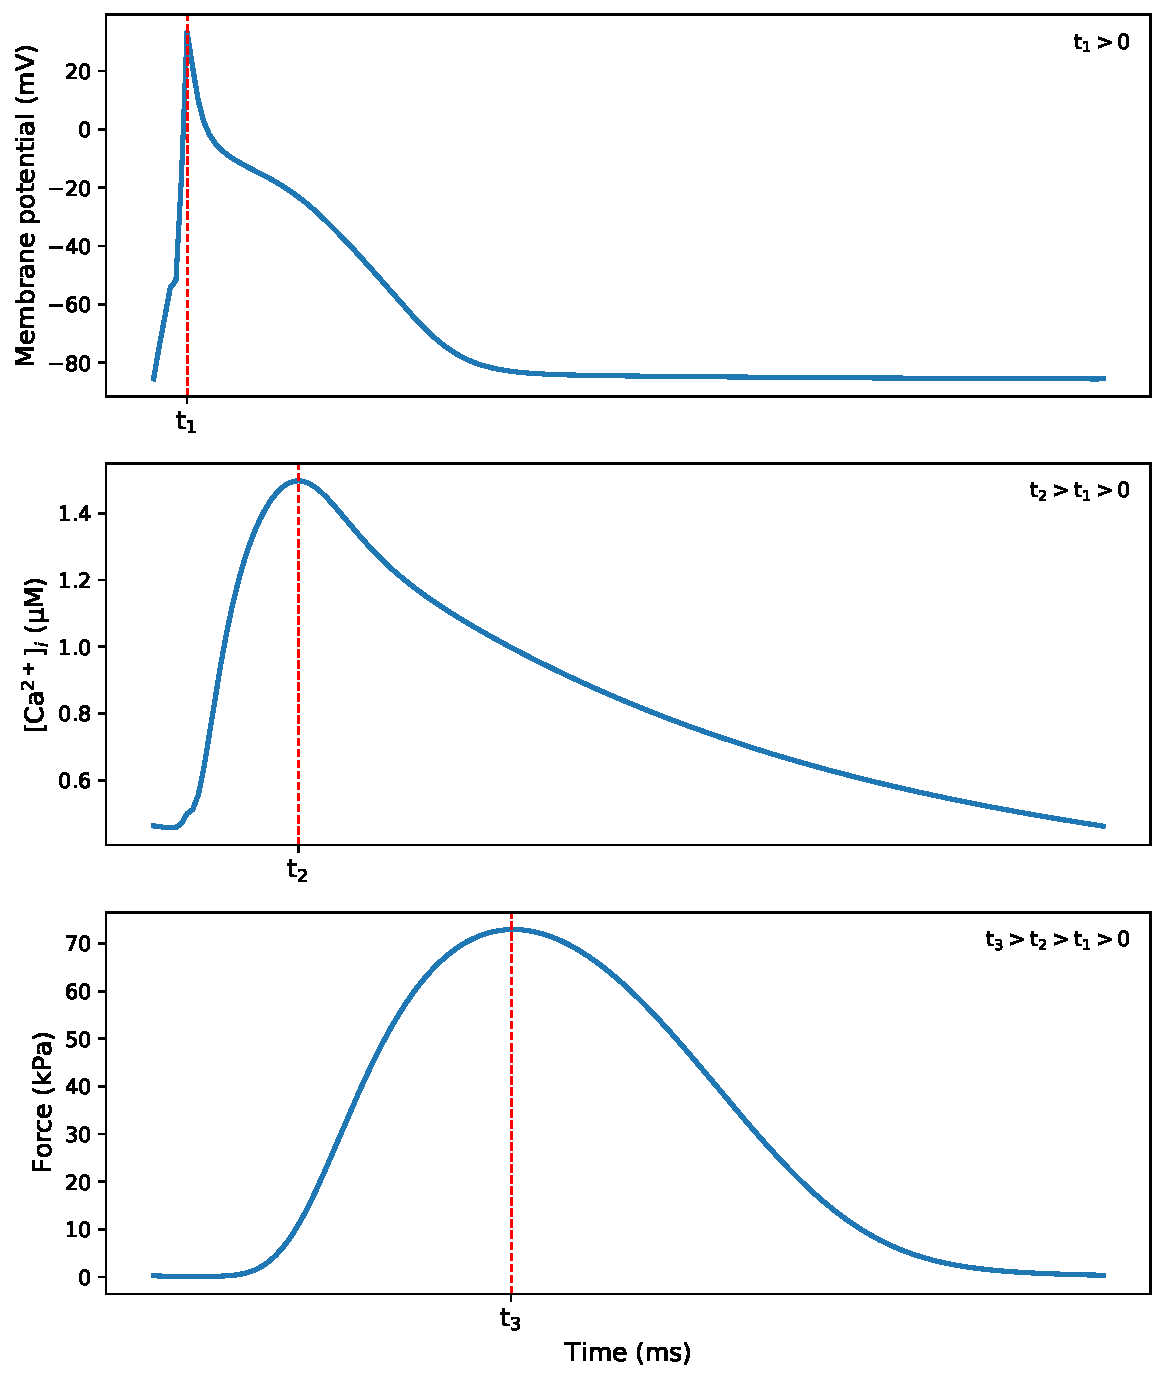
\includegraphics[width=0.66\textwidth]{figures/chapter01/three_peaks.pdf}
    \caption{Example action potential, calcium transient and twitch transient in the rat left ventricular myocyte. From the top to bottom, the three curves are clearly peaking at three successive time points $t_1,\,t_2,\,t_3$.}
    \label{fig:my_label1}
\end{figure}

% [\textbf{TODO}: differences across species]
% Ion currents dynamics may vary a lot across animal species, and this results in different AP shapes, as in the case of humans compared to mice and rats. In Figure~\ref{fig:apcomp}, human and mouse APs are shown. Although most ion channels are conserved across species, there are significant differences in the potassium currents involved in repolarization between human and mouse ventricular myocytes \cite{nerbonne2004}. Specifically, although the upstroke is similar in both species, the repolarization phase shows clear differences. In humans, the upstroke is followed by transient repolarization and a plateau phase, whereas in mice no plateau is visible and repolarization is rapid.

% \begin{figure}
%     \centering
%     \includegraphics[scale=0.4]{figures/ap_human_mouse_comp.png}
%     \caption{Ventricular action potential and currents for human (left) and mouse (right). Credit: \cite{nerbonne2004}}
%     \label{fig:apcomp}
% \end{figure}


% In cardiac myocytes electrical activation elicits an intracellular calcium transient, that in turn signals contraction. 

% Following activation, the L-type Ca channel opens, causing Ca ions to enter the diadic space. Ca ions then bind to  Ryry causing ca induced Ca release from the SR through RyR. Ca diffuses into the cytosol and binds to and actviates the sarcomere. Then as the cell relaxes cytosolic Ca is pumped back up in the SR thrugh SERCATPase and across the cell membrane through the sodium caclicum exchaner and Ca pump 



%
%
%
\subsubsection{The role of calcium in sarcomere contraction}\label{ch1:the_role_of_calcium_in_sarcomere_contraction}
Calcium plays a key role in signalling the cardiac cell to contract. The variation of $\Ca$ levels observed inside the cell during each heart beat is referred to as \textit{calcium transient} or \textit{calcium signal}. To understand the $\Ca$ dynamics that makes the common $\Cai$ transient shape, we need to introduce other important both structural and functional myocyte components.

\vspace{0.2cm}
Cardiac myocytes have a long cylindrical shape. The sarcolemma encapsulating the cell invagenates and forms an extensive tubular network called \textit{transverse} (\acs{T}) \textit{tubules} which allows the AP to penetrate rapidly to the interior of the cell. Next to the T-tubules inside the cell lies the terminal cisternae of the \textit{sarco(endo)plasmic reticulum} (\acs{SR}), forming a closely coupled structure called \textit{dyad}. The SR contains a store of $\Ca$ ions, which are partially released into the \textit{sarcoplasm} (another name for the cytoplasm within the sarcolemma) when the cell is excited. As the AP travels along the sarcolemma and along the T-tubules, $\Ca$ enters the cell through the L-type $\Ca$ channels. $\Ca$ then binds to and activates the \textit{ryanodine receptors} (\acs{RyR}s), which are $\Ca$ release channels located on the SR, triggering further release of a much greater number of $\Ca$ ions from the SR. This process is termed \textit{calcium-induced calcium release}. $\Ca$ diffuses from the dyadic space into the cytosol, and then on the sarcomeric proteins which make up the contractile machinery, activating contraction.

\vspace{0.2cm}
As $\Ca$ is removed from the cytosol, $\Cai$ decreases so that $\Ca$ dissociates from the sarcomeric proteins, causing the sarcomere to relax. $\Ca$ removal is achieved either via $\Ca$ extrusion from the cell or $\Ca$ uptake into intracellular $\Ca$ stores. Two mechanisms are known to be responsible for the extrusion of $\Ca$ from the cell: NCX and the \textit{plasma membrane} $\Ca$ \textit{ATPase} (\acs{PMCA}). The majority of the $\Ca$ entering the cytosol during a $\Cai$ transient is taken up back into the SR via the \textit{sarcoplasmic} $\Ca$ \textit{ATPase} (\acs{SERCA}), with $2$ $\Ca$ ions transported into the SR for every $1$ ATP molecule consumed, returning the cardiac myocyte to its resting state.


%
%
%
\subsection{Cardiac cellular contraction}\label{sec:ch1cardiac_cellular_contraction}
The basic contractile unit of each myocyte is called \textit{sarcomere} and is mainly composed of filamentous proteins (\textit{myofilaments}) between thin partitions called \textit{Z disks}. The two principal interdigitating myofilaments are composed respectively of \textit{myosin} protein (\textit{thick filament}) and of \textit{actin} protein (\textit{thin filament}). The thin filament consists of two actin strings arranged as a two-stranded helix. The groove between the actin strands contains two regulatory proteins: \textit{tropomyosin} (\acs{Tn}) and \textit{troponin} (\acs{Tm}). The sarcomere also contains spring-like filaments of \textit{titin}, connecting Z disks. They ensure that myosin filaments stay aligned and they confer elasticity to the heart wall along with the extracellular \textit{collagen}.

\begin{figure}[!ht]
    \myfloatalign
    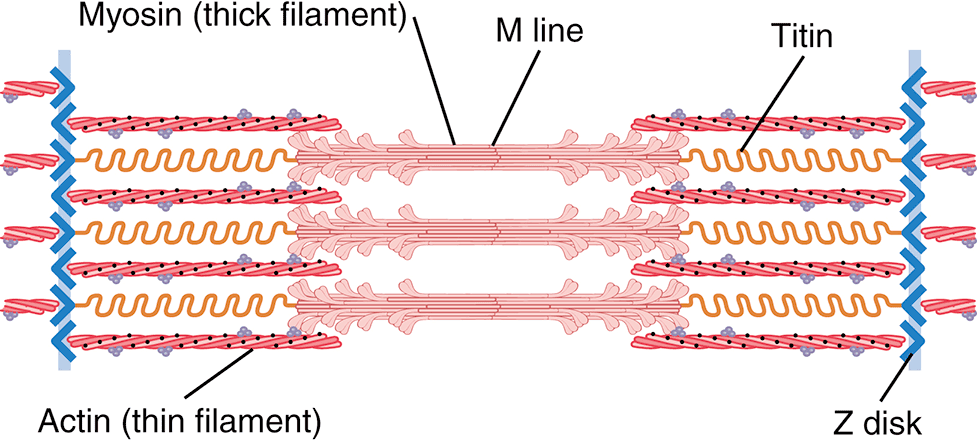
\includegraphics[width=0.66\textwidth]{figures/chapter01/fig_elsv_5.png}
    \caption{Proteins' organisation within the sarcomere. Adapted from~\cite{Guyton:2021}, Unit II, Chapter 6, Page 81, Figure 6-3. Copyright $\textcopyright$ 2021 by Elsevier, Inc.}
    \label{fig:my_label3}
\end{figure}

\vspace{0.2cm}
In the heart, contraction is initiated by a rise in $\Cai$. $\Ca$ binds to the calcium-binding subunit of Tn, namely \textit{troponin C} (\acs{TnC}), on the thin filament, which causes Tm to move out of the actin groove exposing actin binding sites. The thick filament, made of many myosin molecules, has its main body composed by centrally aligned myosin \textit{tails} and protruding myosin \textit{heads} exposed: these can now bind to actin. Contraction then follows as described by the \textit{sliding filament theory}. The attached myosin heads rotate in the \textit{power stoke}, pulling the thick filaments past the thin filaments, causing the sarcomere to contract. The myosin heads then unbind and can reattach to actin to further contract the sarcomere. The acto-myosin bond which is formed through attachment of myosin heads on the actin filament is called \textit{cross-bridge}, and constitutes an independent generator of force: the force generated within the entire sarcomere is therefore proportional to the number of attached myosin heads. 

\begin{figure}[!ht]
    \myfloatalign
    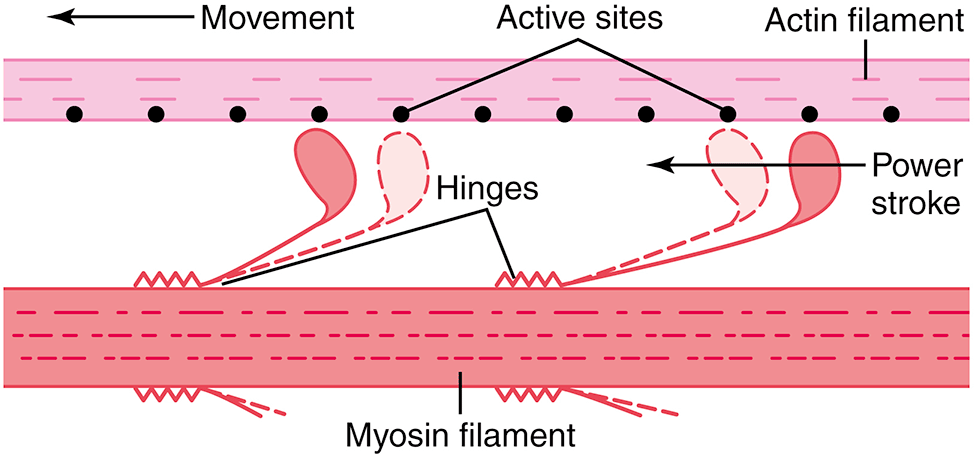
\includegraphics[width=0.66\textwidth]{figures/chapter01/fig_elsv_10.png}
    \caption{The sliding filament mechanisms at the basis of sarcomere contraction. Adapted from~\cite{Guyton:2021}, Unit II, Chapter 6, Page 84, Figure 6-8. Copyright $\textcopyright$ 2021 by Elsevier, Inc.}
    \label{fig:powerstroke}
\end{figure}


% In
% the ventricles, fibre orientation has been known to smoothly rotate
% between endocardium and epicardium ever since original work by
% Streeter (Streeter et al., 1969). This finding obtained by visual
% inspection of tissue has been confirmed using various techniques,
% such as histology (Streeter et al., 1969), optical techniques (Hucker
% et al., 2008; Sands et al., 2005; Smith et al., 2008), and diffusion
% tensor MRI (Gilbert et al., 2007) (Fig. 3). Peskin also used mechanical
% principles to derive the fibre architecture of the ventricles with
% a prediction of about 180  of rotation between endocardium and
% epicardium (Peskin, 1989).

% In addition to the fibrous structure described above, ventricular
% myocytes are organised into laminar structures, also called sheets,
% which were first described in detail by Feneis and Hort (Hort, 1957a,
% 1957b, 1960). These sheets are typically 4e6 myocytes thick and are
% separated by cleavage planes and layers of connective tissue.


%
%
%
\subsection{Cardiac physiologic anatomy}\label{sec:ch1cardiac_physiologic_anatomy}
The heart is composed of two muscular pumps, the right and left ventricles (\acs{RV}, \acs{LV}), each one filled from a contractile reservoir, respectively the right and left atria (\acs{RA}, \acs{LA}). Atrial and ventricular cells are the two major types of cardiac muscle along with His-Purkinje system cells, although the latters are mainly responsable for controlling the rhythmical beating of the heart rather than generating tension. Cardiac muscle cells take the name of \textit{cardiomyoctytes}. As we will not deal with skeletal muscle in this thesis, we will refer to them as simply \textit{myocytes} with no ambiguities.

\vspace{0.2cm}
In the heart, myocytes are joined together at their ends by \textit{intercalated discs} to form long \textit{fibres}. At the intercalated discs, each myocyte effectively connects to a network of electrochemically coupled cells (\textit{syncytium}). This is due to the presence of \textit{gap junctions} where the membranes of two interfacing cells almost fuse with one another, allowing rapid diffusion of ions. Fibers are further arranged into \textit{sheets}, and many sheets form the main layer of the heart walls, namely the \textit{myocardium}, encapsulated within the \textit{endocardium} (internal layer) and the \textit{epicardium} (external layer). The sheets spread within the myocardium in many different and specific directions resulting in the heart contracting in a twisting motion, thereby maximising the amount of blood ejected from the ventricles. The epicardium is the innermost layer of a more complex structure called \textit{pericardium} which surrounds the heart, conferring both structural and mechanical stability and lubrification.

\vspace{0.2cm}
The atria and the ventricles are two distinct functional syncytia, meaning that activation in the atria does not directly pass to the ventricles: this is mediated by the AV bundle (Section~\ref{sec:ch1physiology_of_the_heart}). The two syncytia are in fact separated by fibrous, non-conductive tissue surrounding two openings called \textit{atrio-ventricular valves}. AV valves physically connect the \textit{blood pools} or \textit{chambers} in the left and the right heart enclosed within the atrial and ventricular syncytia. The heart chambers are further connected to the arterial \textit{pulmonary circulation} and \textit{systemic circulation} through the \textit{pulmonary} and \textit{aortic valves}, respectively, and to the venous pulmonary and systemic circulation via four \textit{pulmonary veins} and via the \textit{inferior} and \textit{superior venae cavae} and \textit{coronary sinus}, respectively.

\vspace{0.2cm}
The series of cardiac events that occur in the time frame that goes from the beginning of one heart beat until the beginning of the next are called \textit{cardiac cycle}. This is presented in the next paragraph.


%
%
%
\subsection{Cardiac cycle}\label{sec:ch1cardiac_cycle}
The cardiac cycle consists of a period of relaxation called \textit{diastole}, during which the ventricles are filled with blood from the atria, followed by a period of contraction called \textit{systole}, when the blood is ejected from the ventricles to the lungs, the heart tissue itself and the rest of the body. At each moment of the cardiac cycle, the amount of blood in the heart remains constant, although differently distributed among the four chambers.

\vspace{0.2cm}
Venous blood flows through the systemic and pulmonary venous system major vessels (Section~\ref{sec:ch1cardiac_physiologic_anatomy}) to the RA and LA, respectively. Following spontaneous depolarisation of the SA node myocytes, atria are activated and start contracting, pumping blood into the ventricles. Atrial contraction thus serves as primer pump to ventricular \textit{filling}. The volume of blood in a ventricle at the end of its filling is called \textit{end-diastolic volume} (\acs{EDV}), while the corresponding chamber pressure is called \textit{end-diastolic pressure} (\acs{EDP}). The activation wave then travels through the AV node to the AV bundle, reaching the ventricles in the form of an AP which depolarises the ventricular myocytes, evoking a calcium transient which activates the contractile sarcomeric proteins. Atrial systole is therefore followed by ventricular systole. As the $\Ca$ starts binding to TnC, cross-bridges are formed and active tension is generated, causing a sharp rise in ventricular pressure above the atrial pressure which makes the AV valves close by a reversed pressure gradient, preventing retrograde blood flow. However, as the developed pressure is not yet sufficient to push the aortic and pulmonary valves open, ventricular contraction initially occurs with no emptying. In fact, the force generated within each sarcomere is still not high enough, so that little or no shortening of the muscle fibres is occurring, producing an \textit{isovolumetric contraction} (\acs{IVC}) with further pressure increase. As more cross-bridges are formed, more tension is generated so that the ventricular pressure now exceeds the arterial pressure, making the aortic and pulmonary valves open and causing \textit{ejection} of blood from the ventricles. The ejected blood volume also called \textit{stroke volume} (\acs{SV}) is only about two-thirds of the available EDV of blood: a residual blood volume, namely the \textit{end-systolic volume} (\acs{ESV}), remains. The proportion of ejected blood, i.e. SV divided by EDV, takes the name of \textit{ejection fraction} (\acs{EF}). The ejection rate is initially rapid when the maximum number of cross-bridges are formed and generated tension is at its maximum, and then progressively slows down as $\Ca$ starts dissociating from TnC. Since the rate at which the aortic blood is draining away into the peripheral circulation now exceeds ventricular ejection, ventricular pressure also begins to fall until reaching the \textit{end-systolic pressure} (\acs{ESP}) when the outflow valves close. At this point, both the ventricles become closed chambers again, and a rapid pressure fall occurs driven by the elastic recoil of the deformed and relaxing myocardium. This process takes place at constant blood volumes and is called \textit{isovolumetric relaxation} (\acs{IVR}). When most of the systolic $\Ca$ is extruded from the intracellular space to the ouside or back into the SR, the intraventricular pressures decrease back to their low diastolic levels, the AV valves open and blood floods in from the atria (which have themselves been filling up during ventricular systole) and the next cardiac cycle begins.

\vspace{0.2cm}
To summarise, isovolumetric contraction, ejection, isovolumetric relaxation and filling are the $4$ main phases of the cardiac cycle (Figure~\ref{fig:wiggersdiagram}).

\begin{figure}[!ht]
    \myfloatalign
    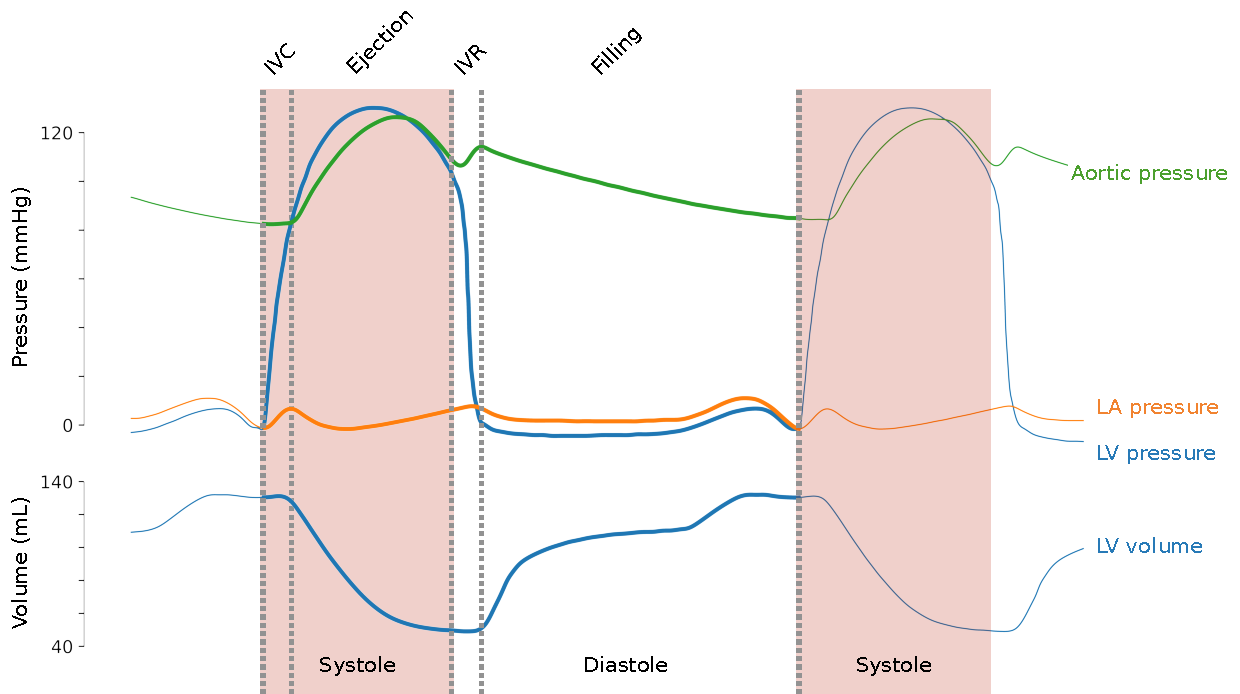
\includegraphics[width=\textwidth]{figures/chapter01/wiggers_diagram.pdf}
    \caption{Wiggers diagram representing the four main phases of the cardiac cycle in the left heart.}
    \label{fig:wiggersdiagram}
\end{figure}


%
%
%
\section{Mathematical modelling of the heart}\label{sec:ch1mathematical_modelling_of_the_heart}
Biophysically detailed mathematical models have been developed to better understand cardiac physiology at different scales of the system, from cell to the whole-organ levels, and to gain insight into the pathophysiology of complex cardiovascular diseases and help interpret clinical observations to improve patients treatment.


%
%
%
\subsection{Cell electrophysiology}\label{sec:cell_ep_modelling}
Models of cardiac cells electrophysiology began with the work of Noble in 1962~\cite{Noble:1962}, who for the first time \textit{in silico} reproduced the long-lasting action and pace-maker potentials of Purkinje fibres of the heart. He continued on the pioneering work of Hodgkin and Huxley~\cite{Hodgkin:1952}, who in 1952 modelled $\Na$, $\K$ and leakage currents across the surface membrane of a squid giant nerve fibre, that give rise to dynamic changes in membrane potential and hence the AP.

\vspace{0.2cm}
The sarcolemma was modelled as an electrical circuit (\textit{equivalent circuit model}), comprised of a capacitor in parallel with resistors that represented ionic currents. The total membrane current was given as the sum of the capacitive current and the ionic current:
%
\begin{equation}\label{eq:membranecurrent}
I_m = C_m\,\der{V_m}{t} + I_i\,,\quad\text{with}\quad I_i = \sum_{\textrm{ion}}I_\textrm{ion}
\end{equation}

\noindent
where

\vspace{0.2cm}
\begin{tabular}{ll}
    $I_m$            & total membrane current \\
    $I_i$            & total ionic current, i.e. sum of all ionic currents $I_\textrm{ion}$ with sign \\
    & (negative, positive for inward, outward currents respectively) \\ 
    $C_m$            & cell membrane capacitance per unit area \\
    $V_m$            & transmembrane voltage
\end{tabular}

\vspace{0.2cm}\noindent
and for each ion species the corresponding transmembrane current $I_{\textrm{ion}}$ was described by the \textit{Ohm's law} as:
%
\begin{equation}\label{eq:ohmslawsinglechannel}
    I_{\textrm{ion}} = g_{\textrm{ion}}\,(V_m-E_{\textrm{ion}})
\end{equation}

\noindent
where

\vspace{0.2cm}
\begin{tabular}{ll}
    $g_{\textrm{ion}}$ & average channel conductance \\
    $E_\textrm{ion}$ & equilibrium potential of the ion
\end{tabular}

\vspace{0.2cm}\noindent
The equilibrium potential of a given ion species is the electric potential that would be required to maintain a zero net ion flux if the ion was allowed to diffuse down to its concentration gradient, assuming the cell membrane being permeable to only that ion species. The \textit{Nernst equation} expresses the equilibrium potential of a ion as a function of the ion concentrations inside and outside the cell:
%
\begin{equation}
    E_{\textrm{ion}}=\frac{\textrm{R}\textrm{T}}{\textrm{F}z}\,\ln{\frac{[\textrm{ion}]_{e}}{[\textrm{ion}]_{i}}}
\end{equation}

\noindent
where

\vspace{0.2cm}
\begin{tabular}{ll}
    $\textrm{R}$  & gas constant \\
    $\textrm{T}$  & absolute temperature \\
    $\textrm{F}$  & Faraday's constant \\
    $z$           & ion valency \\
    $[\textrm{ion}]_{i}$  & ion intracellular concentration \\
    $[\textrm{ion}]_{e}$  & ion extracellular concentration \\
\end{tabular}

\vspace{0.2cm}
Since Noble's work, many ionic cell models have been developed to represent the baseline physiology of both atrial, ventricular, and SA node myocytes~\cite{Corrado:2020}. These many currently available models all share the same cell membrane modelling strategy by viewing it as an electric circuit (equation~\eqref{eq:membranecurrent}), and mostly differ in single ion channels' kinetics representation.

\vspace{0.2cm}\noindent
The current $I_{\textrm{ion}}$ introduced in equation~\eqref{eq:membranecurrent} is the result of ions moving across the cell membrane through an ion channel, which is made of pore-forming proteins that span the membrane lipid bi-layer. Ion channels are regulated by one or more \textit{gates}, which allow ions to pass according to whether they are in an open or closed state. Changes in an ion channel conformation takes place in response to chemical or electrical signals, temperature, or mechanical stress. Cardiac cells ion channels are mostly \textit{voltage-gated}, meaning that they change conformation with varying transmembrane voltage. Two approaches are commonly being used to represent ionic channels kinetics: the first uses the Hodgkin-Huxley (\acs{HH}) formulation~\cite{Hodgkin:1952} while the second (a generalisation of the first) uses continuous-time Markov chain models (\acs{MM})~\cite{Fink:2009}.

\vspace{0.2cm}
In the HH characterisation of channels, the conductance $g_{ion}$ (equation~\eqref{eq:ohmslawsinglechannel}) is given by the product of a maximal conductance term and one or more separate \textit{gating variables} that represent the probability of finding the channel open:
%
\begin{equation}
    g_{\textrm{ion}} = g_{\textrm{ion}}^{\textrm{max}}\times y_i\cdot\dots\cdot y_N
\end{equation}

\noindent
where each gating variable $y:=y_i$ can be formulated using the equation:
%
\begin{equation}
    \der{y}{t} = \frac{y_{\infty}-y}{\tau_y}
\end{equation}

\noindent
where

\vspace{0.5cm}
\begin{tabular}{ll}
$y_{\infty}$ & voltage-dependent steady-state function of the gate \\
$\tau_{y}$ & voltage-dependent time constant
\end{tabular}

\vspace{0.5cm}
\noindent
The gating variables described in the HH formulation do not represent specific kinetic states of the ion channel. Moreover, they are assumed to be independent.

\vspace{0.2cm}
To accurately describe the dependence of a given transition on the occupancy of different states for a given channel, MMs are used. In this case, a discrete number of states represent the possible configurations a channel has. Transitions from one state to the other can occur at different rates, and the rate zero is used by convention when no direct switching between two given states is possible. Gating variables will then simply represent the probability of finding the channel in the respective states (\textit{state variables}). An example of MM approach to model an ion channel which can be either in the open, closed or inactivated configuration includes $3$ state variables to represent the three possible configurations and $6$ transition rates. Variation of state $y_i$ is given as a function of the other state variables $y_j$ for $j\in\{1,2,3\}\setminus{\{i\}}$:
%
\begin{equation}
    \der{y_i}{t} = \sum_{\substack{j=1 \\ j\neq i}}^{3} (k_{ji}\,y_j-k_{ij}\,y_i)
\end{equation}

\noindent
were $k_{ji}\in\mathbb{R}$ is the rate at which transition from state $y_j$ to state $y_i$ occurs.

\vspace{0.5cm}
It is worth mentioning that the two presented HH and MM modelling frameworks are not mutually exclusive but are instead very frequently used in combination to represent the many different ion channels within the cell.

% \vspace{0.2cm}
% \cite{hinch2004, pandit2001, gattoni2016}. In this study, the rat ventricular electrophysiology and calcium dynamics are described by employing Gattoni et al. \cite{gattoni2016} model, fitted to consistent experimental data in both SHAM and AB rats at physiological frequency and temperature \cite{gattoni2017}.


%
%
%
\subsection{Cell contraction}\label{sec:cell_contr_modelling}
Cardiac contraction models are used to simulate active tension generation at the sarcomere level arising from the thin and thick filaments. Development of these models has proceeded over the years in parallel with key experimental discoveries about striated and cardiac muscle physiology~\cite{Niederer:2019}. Contraction models have transitioned from simple phenomenological models aiming to represent the average sarcomere dynamics to very complex, spatially detailed models trying to capture the explicit positions of individual molecules. However, in the view of incorporating these models within whole-organ computational frameworks, currently adopted sarcomere contraction models have achieved a balance between recapitulating the main mechanistic phenomena while still being represented by a tractable number of ordinary differential equations (\acs{ODE}s) to remain computationally efficient to solve. Key mechanisms that are desirable to recapitulate in these multi-scale sarcomere contraction models include force dependence on sarcomere length (\textit{Frank-Starling mechanism}), myofilament cooperative activation by $\Ca$, acto-myosin cooperative interaction in crossbridges formation and force dependence on sarcomere length variation (velocity).

% Models have been developed with a wide spectrum of complexity, going from the will of capturing the explicit positions of individual molecules to simply aiming to represent the average sarcomere dynamics \cite{Niederer:2019}. Whole organ modelling relies on the latter models, due to their computational efficiency. An example of this kind of models is given by the rat heart contraction model developed by Land et al. \cite{land2012a}, based on the relevant two works of Niederer, Hunter $\&$ Smith \cite{niederer2006} and Rice, Wang $\&$ de Tombe \cite{rice2008}. This model simulates troponin C, tropomyosin and crossbrigde dynamics and predicts the tension generated by cardiac muscle in response to changes in $\Ca$, length and velocity. 

% %
% %
% %
% \vspace{0.5cm}
% \textbf{Modelling $\Ca$ dependence}

% \vspace{0.2cm}
% The Land et al. \cite{land2012a} equation for troponin binding captures the cooperativity experimentally observed in calcium binding to the second binding site on troponin C (TnC), and has a Hill curve as steady-state solution:

% \begin{equation}\label{eq:trpneq}
%     \frac{d\trpn}{dt} = k_{\trpn}\,\left[\left(\frac{\Cai}{\Caift}\right)^{n_{\trpn}}(1-\trpn)-\trpn\right]
% \end{equation}

% where $\trpn$ represents the fraction of occupied regulatory sites, $k_{\trpn}$ the unbinding rate and $n_{\trpn}$ the Hill coefficient. The process of calcium binding to TnC causes a conformational change in its associated tropomyiosin complex, unblocking the actin sites for myosin crossbridge cycling. In Land et al. work, differently from the previous work of Rice et al. \cite{rice2008}, the crossbridge cycle has been collapsed to a single state, yielding a model with only two states: (1) the crossbridge state $\xb$ in which the crossbridge is actively cycling, and (2) the non-permissive state $1-\xb$. As in equation~\ref{eq:trpneq}, also the expression for the transition between these two states has been chosen to give a Hill curve in the steady-state:

% \begin{equation}\label{eq:xbeq}
%     \dfrac{d\xb}{dt} = \kxb\,\left[\permtot\,(1-\xb)-\frac{1}{\permtot}\,\xb\right]
% \end{equation}

% where

% \begin{equation}
%     \permtot := \sqrt{ \left( \frac{\trpn}{\trpnf} \right) ^{\nxb} }
% \end{equation}

% and being $\kxb$ the unbinding rate and $\nxb$ the Hill coefficient.

% % \begin{figure}[H]
% %     \centering
% %     \includegraphics[width=0.6\textwidth]{figures/land_et_al.png}
% %     \caption{Framework of the cell contraction model and its interaction at tissue scale in Land et al. model \cite{land2012a}.}
% % \end{figure}

% %
% %
% %
% \vspace{0.5cm}
% \textbf{Length- and velocity-dependence}

% \vspace{0.2cm}
% For developing models of cardiac muscle, detailed data on the velocity-dependent response are often required. These data are fitted to the function proposed by Kawai et al. \cite{kawai1993}:

% \begin{equation}\label{eq:eqkawaii}
%     y(f) = H - \frac{B\,i\,f}{b+i\,f}+\frac{C\,i\,f}{c+i\,f}+\frac{D\,i\,f}{d+i\,f}
% \end{equation}

% In the Land et al. model \cite{land2012a}, length- and velocity-dependent processes were taken into account in the normalized generated force expression as follows:

% \begin{equation}\label{eq:normforce}
%     F_n = g(Q)\cdot h(\lambda)\cdot \xb
% \end{equation}

% where $g(Q)$ determines the velocity dependence and $h(\lambda)$ the change in maximum force, being $\lambda$ the extension ratio along the fibre direction. The increase in maximum force was based on filament overlap and modelled using the same approach adopted by Rice et al. \cite{rice2008}:

% \begin{align}
%     h'(\lambda) &= 1+\beta_0\,[\lambda+\min(\lambda,\,0.87)-1.87] \\
%     h(\lambda) &= \max(0,\,h'(\min(\lambda,\,1.2)))
% \end{align}

% where $\beta_0 = 1.65$, resulting in a linear length dependence near resting length, and a twice as steep decrease in tension when the sarcomere length falls below the thick filament length (at $\lambda = 0.87$). A shift in calcium sensitivity is an additional and important mechanism for the length-dependence of tension. They used a simple phenomenological representation of it, where the calcium sensitivity $\Caift$ is directly length-dependent:

% \begin{equation}
%     \Caift = \Caift^{\text{ref}}\,(1+\beta_1\,(\lambda-1))
% \end{equation}

% where $\beta_1$ is then fitted based on experimental data. The parametrization of the velocity dependence was based on sinusoidal analysis experiments (Kawai and Brandt \cite{kawai1980}), but fitting an equation different from~\eqref{eq:eqkawaii} coming from the work of Palmer et al. \cite{palmer2007}, where the \textit{D process} is dropped and a more detailed fit to passive tension is used.

% \vspace{0.5cm}
% Whereas length dependence can often be represented by a modification to binding rates or scaling of force, the complex response to shortening velocity requires a more detailed model. As previously done in Niederer et al. \cite{niederer2006}, the \textit{fading memory model} (FMM) was employed to represent the velocity response as several strain-rate-dependent variables decay with time. An advantage of this model is that it is independent of the contraction model, as it can be added as an addition after modelling isometric tension and length-dependence. Use of the FMM model allows the tension development dependence on crossbridge kinetics to be phenomenologically represented. It describes the relationship between tension and sarcomere sliding velocity, by separating tension development into a non-linear static component and a linear time-dependent component.

% \vspace{0.5cm}
% The FMM model introduces two equations of the form:

% \begin{equation}
%     \der{Q_i}{t} = A_i\,\der{\lambda}{t}-\alpha_i\,Q_i
% \end{equation}

% The $A_i$ parameters are directly related to the viscous and elastic moduli, and $\alpha_i$ to the frequencies. Parameters $\alpha_1,\, A_1$ are related to the slower "B process", and $\alpha_2,\,A_2$ to the faster "C process". The effect $g(Q)$ seen in equation~\eqref{eq:normforce} on tension is given by an equation derived from the Hill force-velocity curve extended to model stretch and shortening in a symmetric way \cite{niederer2006}:

% \begin{equation}
%     g(Q) = \begin{cases}
%         \dfrac{a\,Q+1}{1-Q}\qquad & Q\le 0 \\
%         \dfrac{1+(a+2)\,Q}{1+Q}\qquad & Q>0
%     \end{cases}\qquad\text{where}\quad Q = \sum_{i=1}^2 Q_i
% \end{equation}

% and $a$ is the slope of Hill force-velocity equation.

% \vspace{0.5cm}
% Finally, tension was scaled from normalized force to actual tension for a whole organ context:
% \begin{equation}
% T_a =T_{ref}\cdot F_n
% \end{equation}
% where the reference tension $T_{ref}$ encapsulates the total number of crossbridges and the fraction of cycling crossbridges in the force generating state at any time.


%
%
%
\subsection{Electromechanical coupling}\label{sec:mathelecmechcoupl}
In biophysically detailed models of cardiac electromechanics, the active tension along the muscle fibres direction is calculated using sarcomere contraction models, introduced in Section~\ref{sec:cell_contr_modelling}. This calculation is normally performed in two steps. The first step consists in solving a system of ODEs of the form:
%
\begin{equation}\label{eq:epmechcoupling}
    \der{\mathbf{y}}{t} = f(t,\,\lambda,\,\dot{\lambda},\,\mathbf{y}) 
\end{equation}

\noindent
where $f$ is a generic non-linear function and

\vspace{0.2cm}
\begin{tabular}{ll}
    $t$             & time \\
    $\lambda$       & fibre strain \\
    $\dot{\lambda}$ & fibre strain rate ($=\mathrm{d}\lambda / \mathrm{d}t$) \\
    $\mathbf{y}$    & vector of state variables
\end{tabular}

\vspace{0.2cm}\noindent
In the second step, active tension ($T_a$) is calculated as a function of time, fibre strain and strain rate and state variables which are varying over time, via a generic non-linear function $h$:
%
\begin{equation}\label{eq:activetensioncalc}
    T_a = h(t,\, \lambda,\,\dot{\lambda},\,\mathbf{y}) \\
\end{equation}

\vspace{0.2cm}
The coupling between the electrical and mechanical components of the model resides in the definition of the vector of state variables $\mathbf{y}$. In fact, this is in part given by the cell electrophysiology model components (gate and/or state variables) and in part given by the cell contraction model components (thin and thick filament proteins). The variation in the second components can depend on the current state of the first components. The most common example sees $\Ca$ binding to TnC which triggers the sarcomere to contract (Section~\ref{sec:ch1cardiac_cellular_contraction}). In this case, the current state of the electrophysiology model ($\Cai(t)$ for a fixed $t$) directly affects the variation in the $\Ca$-TnC bound complexes and consequently in the cross-bridge formation.


%
%
%
\subsection{Tissue electrophysiology}\label{sec:tissue_ep_math_modelling}
A tissue model of cardiac electrophysiology is required to link cellular excitation through to whole organ electrical activation.

\vspace{0.2cm}
When a single cardiac myocyte undergoes depolarisation, the evoked AP travels in the form of a depolarisation wave which is able to activate the neighbouring cells. We have seen that cardiac myocytes are microscopically organised into fibres, and further organised into sheets (Section~\ref{sec:ch1cardiac_physiologic_anatomy}). This peculiar spatial arrangment causes an anisotropic propagation of the depolarisation wavefront, which is faster along the principal axis of the fibre and slower in the other directions. Different factors can affect propagation, including the shape of the myocytes, the curvature of the wavefront, the relative positions of the gap junctions within the fibres, the extracellular matrix composition and the local vasculature~\cite{Clayton:2011}. In the $3$-dimensional ventricular tissue, the AP depolarisation wave propagation is mainly orthogonal, with the fibre, sheet, and sheet-normal being the three principal directions.

\vspace{0.2cm}
Cardiac tissue electrophysiology can be mathematically described by first considering the tissue as a syncytium of electrically coupled cells, and successively homogenising it to treat it as a smooth, continous space. In the \textit{bidomain model}, both the intracellular (subscript $i$) and the extracellular (subscript $e$) spaces are considered as smooth and overlapping domains, separated by the cell membrane. The electric current densities in the two domains are described by the Ohm's law as:
%
\begin{equation}\label{eq:ohmslaw}
    \mathbf{J}_{\text{d}} = -\mathbf{G}_{\text{d}}\nabla\phi_{\text{d}}\,,\quad\text{with}\quad \text{d}=i,\,e
\end{equation}

\noindent
where

\vspace{0.2cm}
\begin{tabular}{ll}
    $\mathbf{\mathbf{J}_{\text{d}}}$ & current density \\
    $\mathbf{G}_{\text{d}}$ & conductivity tensor \\
    $\phi_{\text{d}}$ & electric potential \\
\end{tabular}

\vspace{0.2cm}\noindent
Conservation of current and charge is then enforced:
%
\begin{equation}
    \begin{aligned}
        & \nabla\cdot\mathbf{J}_i = -I_m \\
        & \nabla\cdot\mathbf{J}_e =  I_m \\
    \end{aligned}\quad\Rightarrow\quad \nabla\cdot(\mathbf{J}_i+\mathbf{J}_e) = 0
\end{equation}

\noindent
where $I_m$ is the cell membrane current calculated as in equation~\eqref{eq:membranecurrent} using an ionic cellular model (Section~\ref{sec:cell_ep_modelling}), and additionally scaled by a factor $\beta_m$ to match the domains' $3$-dimensional nature:
%
\begin{equation}\label{eq:membranecurrentsc}
    I_m = \beta_m\left(C_m\,\der{V_m}{t} + I_i\right)
\end{equation}

\noindent
The transmembrane voltage can be expressed in terms of electric potentials as
%
\begin{equation}
    V_m = \phi_i - \phi_e
\end{equation}

\noindent
so that the final set of equations describing the bidomain model takes the following form:
%
\begin{align}\label{eq:bidomainmodel}
    & \nabla\cdot(\mathbf{G}_i(\nabla V_m + \nabla \phi_{\text{e}})) = \beta_m\left(C_m\,\der{V_m}{t} + I_i\right) \\
    & \nabla\cdot((\mathbf{G}_i + \mathbf{G}_e)\nabla \phi_e) = -\nabla\cdot(\mathbf{G}_i\nabla V_m)
\end{align}

\noindent
The system is solved using the finite element method with no-flux conditions at the computational domain boundaries (\textit{Neumann boundary conditions}). $\mathbf{G}_i$ and $\mathbf{G}_e$ conductivity tensors' components are taken to reflect the anisotropy of the cardiac tissue.


%
%
%
\subsection{Tissue mechanics}\label{sec:tissue_mech_math_modelling}
A tissue model of cardiac mechanics is required to link cellular active contraction models through to whole organ pump function. For the modelling of the mechanical properties of cardiac tissue non-linear solid mechanics is used.

\vspace{0.2cm}
Like electrical properties, tissue mechanical properties depend on the orientation of cardiac tissue microstructure. Therefore, to mathematically describe cardiac tissue deformations, tensors are commonly given in terms of a coordinate system locally aligned with the muscle fibre ($\mathbf{f}$), sheet ($\mathbf{s}$) and sheet-normal directions ($\mathbf{n}$) in the reference configuration, determining the orthonormal matrix $\mathbf{L} = [\mathbf{f}\,\mathbf{s}\,\mathbf{n}]$. In finite elastic deformation theory, the transformation from undeformed ($\mathbf{X}$) configuration to deformed ($\mathbf{x}$) configuration is described by means of the deformation gradient tensor:
%
\begin{equation}
    \mathbf{F} = \frac{\partial \mathbf{x}}{\partial\mathbf{X}}
\end{equation}

\noindent
The determinant of the deformation gradient $J:=\text{det}(\mathbf{F})$ measures the volume variation as the material undergoes deformation. Large deformation mechanics equations for an incompressible solid enforce the stress equilibrium with an incompressibility constraint:
%
\begin{equation}
    -\nabla\cdot(\mathbf{F}\mathbf{T}) = 0\,,\quad\text{with constraint}\quad J = 1
\end{equation}

\noindent
where $\mathbf{T}$ is the second Piola-Kirchhoff stress tensor. The solution to the mechanics problem requires a description of the material behaviour known as the \textit{constitutive law}~\cite{BonetWood:2008}, which gives the stress tensor $\mathbf{T}$ as a function of the Green strain tensor $\mathbf{E}$ and the Cauchy strain tensor $\mathbf{C}$ for the material. The Green strain tensor is given as a function of the deformation gradient tensor:
%
\begin{equation}
    \mathbf{E} = \frac{1}{2}\,(\mathbf{C}-\mathbf{I})\,,\quad\text{with}\quad \mathbf{C}=\mathbf{F}^T\mathbf{F}
\end{equation}

\noindent
and is transformed to a fibre-aligned coordinate system using $\mathbf{E^{fsn}}=\mathbf{L}^T\,\mathbf{E}\,\mathbf{L}$. The stress tensor $\mathbf{T^{fsn}}$ is determined from the constitutive law, which is generally expressed as a \textit{strain energy function} $W$:
%
\begin{equation}
    \mathbf{T^{fsn}} = \derp{W}{\mathbf{E^{fsn}}}
\end{equation}

\noindent
The stress tensor $\mathbf{T^{fsn}}$ is then transformed back using $\mathbf{L}\,\mathbf{T^{fsn}}\,\mathbf{L}^T$. The final second Piola-Kirchhoff stress tensor is obtained from the strain energy function by adding an active tension component $T_a$ (Section~\ref{sec:cell_contr_modelling}) along the fibres direction $\mathbf{f}$:
%
\begin{equation}\label{eq:eqce}
    \mathbf{T} = \mathbf{L}\,\derp{W}{\mathbf{E^{fsn}}}\,\mathbf{L}^T + T_a\,\mathbf{ff}^T
\end{equation}

\noindent
$\mathbf{T}$ expresses the stresses in actively contracting incompressible cardiac tissue in terms of its strain and completes the set of equations required to model actively contracting cardiac tissue. The resulting system of equations is solved using the finite element method. A given displacement can be used to prescribe the position of the nodes at the computational domain boundaries (\textit{Dirichlet boundary conditions}).


%
%
%
\subsection{Hemodynamics}\label{sec:hemodynamics_math_modelling}
The blood pumped by the heart appears in electromechanical models as a mechanical boundary condition for the cavity pressure. During ejection, the change in pressure can be simulated using a Windkessel model~\cite{Westerhof:1971}. This framework models the aorta as a compliant vessel, which obeys
%
\begin{equation}\label{eq:firstwkelem}
    p_{\textrm{ao}} = \frac{v_{\textrm{ao}}}{C}
\end{equation}

\noindent
where

\vspace{0.2cm}
\begin{tabular}{ll}
    $C$ & total arterial compliance \\
    $p_{\textrm{ao}}$ & aortic blood pressure \\
    $v_{\textrm{ao}}$ & aortic blood volume \\
\end{tabular}

\vspace{0.5cm}
\noindent
Blood flow to the body is modelled using the simple \textit{Darcy's law of flow} which gives the flow as being proportional to the pressure drop between inlet and outlet pressures:
%
\begin{equation}\label{eq:secondwkelem}
    I_{\textrm{out}} = \frac{p_{\textrm{ao}}-p_{\textrm{out}}}{R} 
\end{equation}

\noindent
where

\vspace{0.2cm}
\begin{tabular}{ll}
    $R$ & peripheral body vessels resistance \\
    $I_{\textrm{out}}$ & blood flow to the body \\
    $p_{\textrm{out}}$ & external pressure \\
\end{tabular}

\vspace{0.5cm}
\noindent
The external pressure $p_{\textrm{out}}$ is assumed to be approximately equal to zero. Equations~\eqref{eq:firstwkelem}--\eqref{eq:secondwkelem} make up the \textit{two-element Windkessel model}. However, more realistic aortic pressure waves can be obtained by introducing a second resistance for the aortic valve, making up the \textit{three-element Windkessel model}:
%
\begin{align}\label{eq:windk}
    \der{v_{\textrm{LV}}}{t} &= \frac{1}{Z}\,(p_{\textrm{ao}}-p_{\textrm{LV}}) \\ 
    \der{v_{\textrm{ao}}}{t} &= -I_{\textrm{out}}-\der{v_{\textrm{LV}}}{t} \\
    I_{\textrm{out}} &= \frac{1}{R}\,p_{\textrm{ao}} \\
    p_{\textrm{ao}} &= \frac{1}{C}\,v_{\textrm{ao}}
\end{align}

\noindent
where

\vspace{0.2cm}
\begin{tabular}{ll}
    $Z$ & aortic characteristic impedance \\
    $p_{\textrm{LV}}$ & left-ventricular pressure \\
    $v_{\textrm{LV}}$ & left-ventricular volume
\end{tabular}

\vspace{0.5cm}
\noindent
The three-element Windkessel model equations can also be re-written more concisely as:
%
\begin{equation}\label{eq:windkconcise}
    \dder{v_{\textrm{LV}}}{t} = -\left(\frac{1}{C\,Z}+\frac{1}{R\,C}\right)\,\der{v_{\textrm{LV}}}{t}-\frac{1}{C\,Z\,R}\,p_{\textrm{LV}}-\frac{1}{Z}\,\der{p_{\textrm{LV}}}{t}
\end{equation}

\vspace{0.2cm}
Equation~\eqref{eq:windkconcise} can be further generalised to model simple hemodynamic boundary conditions during the other cardiac cycle phases as well, namely preload filling (to initialise the heart to a prescribed end-diastolic pressure), isovolumetric contraction, isovolumetric relaxation and diastolic filling:
%
\begin{equation}\label{eq:windkgeneral}
    m_1\,\dder{v_{\textrm{LV}}}{t} + m_2\,\der{v_{\textrm{LV}}}{t} + m_3\,\der{p_{\textrm{LV}}}{t} + m_4\,v_{\textrm{LV}} + m_5\,p_{\textrm{LV}} +  m_6 = 0
\end{equation}

\noindent
This is done by solving~\eqref{eq:windkgeneral} with coefficients  $\mathbf{m}:=(m_1,\,\dots,\,m_6)\in\mathbb{R}^6$ adjusted according to the phase in the cardiac cycle as follows:
%
\begin{equation}
    \mathbf{m} = \begin{cases}
    (0,\,0,\,1,\,0,\,0,\,0) & \rightarrow\quad\text{phase $0$: preload filling} \\
    (0,\,1,\,0,\,0,\,0,\,0) & \rightarrow\quad\text{phase $4$: isovolumetric contraction} \\
    (ZC,\,1+Z/R,\,C,\,0,\,1/R,\,0) & \rightarrow\quad\text{phase $1$: systolic ejection (equation~\eqref{eq:windkconcise})} \\
    (0,\,1,\,0,\,0,\,0,\,0) & \rightarrow\quad\text{phase $2$: isovolumetric relaxation} \\
    (0,\,0,\,1,\,0,\,\kappa_{\textrm{diast}},\,-p\cdot \kappa_{\textrm{diast}}) & \rightarrow\quad\text{phase $3$: diastolic filling}
    \end{cases}
\end{equation}

\noindent
Briefly, the heart is inflated to a prescribed end-diastolic pressure ($p$) and stays in the diastolic phase ($\textrm{d}p_{\textrm{LV}}/\textrm{d}t=0$) until volume flow reverses. Next, isovolumetric contraction is simulated ($\textrm{d}v_{\textrm{LV}}/\textrm{d}t=0$) until the cavity pressure is high enough to open the aortic valve (prescribed $p_{\textrm{ao}}$ pressure). Ejection is simulated using the three-element Windkessel model~\eqref{eq:windkconcise}. When flow reverses once again, the constraint for isovolumetric relaxation is set ($\textrm{d}v_{\textrm{LV}}/\textrm{d}t=0$). When pressure finally relaxes below the prescribed $p$, a simple phenomenological model is used for diastole at a fixed $\kappa_{\textrm{diast}}$ inflation speed ($\textrm{d}p_{\textrm{LV}}/\textrm{d}t=\kappa_{\textrm{diast}}\,(p - p_{\textrm{LV}})$).


%
%
%
\section{Heart failure}\label{sec:ch1heart_failure}
Heart failure (\acs{HF}) affects $920,000$ people in the UK \cite{Bhf:2021} and increases the risk of cardiovascular disease, stroke and death \cite{Adelborg:2017, Henkel:2008}.


%
%
%
\subsection{HF with reduced ejection fraction}
HF can be accompanied by a systolic dysfunction, where the ventricular myocytes cannot contract properly and the pumped blood is insufficient to meet the oxygen body demand. This pathological condition is referred to as \textit{heart failure with reduced ejection fraction} (\acs{HFrEF}).


%
%
%
\subsection{HF with preserved ejection fraction}
HF can be accompanied by a diastolic dysfunction, where the ventricular myocytes retain the ability to contract, but cannot relax properly: this pathological condition is referred to as \textit{heart failure with preserved ejection fraction} (\acs{HFpEF}).

\vspace{0.2cm}
HFpEF is a heterogeneous disease mainly attributed to LV diastolic dysfunction. Diastolic function worsens as part of normal ageing \cite{Andersen:2014} and this likely explains much of the age-association with increasing HFpEF risk. Other potentially prominent risk factors for HFpEF include obesity, metabolic syndrome, hypertension, sedentary state, coronary disease, kidney disease~\cite{Pfeffer:2019}. Hypertension is the dominant substrate upon which HFpEF develops, being present in $\SI{80}{\percent}-\SI{90}{\percent}$ of patients in community-based studies e.g.~\cite{Borlaug:2009}. Diastolic dysfunction can be broadly dichotomised into impairments in the \textit{active} and \textit{passive} processes. Active relaxation refers to the rate of pressure decay during isovolumetric relaxation mediated by $\Ca$ re-uptake into the SR, which facilitates detachment in the actin-myosin complex within the cardiomyocyte. In HFpEF, there is an inability to enhance early diastolic relaxation and suction with exercise, contributing to increased filling pressures. There is also an increase in passive LV chamber stiffness in HFpEF, so that even if relaxation and suction were adequate, a higher filling pressure would be required to distend the chamber to an adequate preload volume. This increase in LV passive stiffness is related to changes in the extracellular matrix due to deposition of collagen (\textit{fibrosis})~\cite{Burlew:2002}, as well as changes within the cardiac myocyte, specifically abnormalities in $\Ca$ handling and in the isotype and phosphorylation status of titin sarcomeric macromolecule. Typical structural changes associated with HFpEF are left atrial (LA) enlargement and LV hypertrophy, characterised by an enlargement or thickening of the heart muscle~\cite{Zile:2004}, although investigations in broader HFpEF samples have established a much more heterogeneous cardiac phenotype, characterised by many patterns of cardiac remodelling including no remodelling at all~\cite{Shah:2012}.


%
%
%
\section{Motivation and goals}\label{sec:ch1motivation_and_goals}


%
%
%
\subsection{Quantitatively linking cell, tissue and hemodynamic properties to whole heart function}


%
%
%
\subsection{\textit{In silico} identification of potential pharmacological targets for HF treatment}
Current treatments for HFpEF include angiotensin-converting enzyme inhibitors/aldosterone receptor blockers, calcium channel
blockers and beta-blockers, but the mortality and the morbidity associated with the
disease have so far remained high~\cite{Adamczak:2020}. This may be due to the disparateness of the disease as well as its multifactorial pathophysiology. Therefore, current pharmacotherapies are not effective and patients with HFpEF are
currently considered the largest unmet need in cardiology. At present, there is no cure for HFpEF~\cite{Owan:2006}.

\vspace{0.2cm}
It is known that changes in cardiac contraction that give rise to HFpHF are potentially driven by altered electrophysiology, for example a prolongation in the AP can alter contractile function and a mishandling of $\Ca$ ions can alter the signal received by the sarcomere \cite{Asp:2013, Gorski:2015}. Quantitatively mapping changes in one part of this system to another to understand their role in disease or predicting how changing a single protein's function may affect whole organ function is complex and is not susceptible to intuitive analysis. For this reason, the main purpose of this project is to develop a computational framework to quantitatively link pathological and pharmacological manipulations across scales and physics in the heart. To do this, we propose to build a biophysically detailed $3$D mathematical model of the rat heart. By improving our understanding of the transduction of the electrical signal and sarcomere function through to whole organ contraction in healthy and diseased states, we hope to identify potential targets for treating HFpEF.





%
%
%
\section{Summary}\label{sec:ch1summary}
\todo{write}







% Whole heart contraction is the result of complex molecular mechanisms and electromechanical events at the cellular level. The organ-scale function is thus strongly dependent on and can be manipulated by molecular and cellular events, yet a mapping between cell and organ functions is complex and nonlinear. 
% We aim to quantify this interaction using mathematical models.

% \subsection{Goal}
% Fitting a heart model to experimental data remains a massive challenge. Bayesian history matching (HM) technique has been shown to be a valuable approach for global parameter inference when fitting models of high-dimensional parameter spaces. HM is an iterative process that reduces the model's input space by discarding regions that are unlikely to match experimental data. HM commonly makes use of Gaussian processes (GPs) which are computationally efficient surrogates of the model. Previously employed for fitting models of galaxy formation \cite{Vernon:2010}, infectious disease transmission \cite{Andrianakis:2015}, plant physiology \cite{Vernon:2018} and lately human atrial cell \cite{Coveney:2018}, HM has never been applied (to our knowledge) in the context of whole organ cardiac models nor multi-physics problems.

% \vspace{0.5cm}
% In this study, we employ mathematical models to quantitatively characterise the impaired AB rat left ventricle's contractility function (organ level) and we aim to identify potential drug targets within our in-silico environment that can recover cardiac function by manipulating the calcium dynamics. The degree of recovery will be established according to reference sham-operated (SHAM) rat hearts. In order to achieve this, we made use of computational models of heart electrophysiology and calcium dynamics, sarcomere contraction and mechanics derived from SHAM and AB real ventricles geometries. We firstly match our mathematical model of the heart to experimental data from control and aortic-banded rat hearts. We then propose to use this modelling framework to predict drug targets that can be manipulated to recover cardiac function in the aortic-banded rat heart models, bringing them back closer to the control models.

% \vspace{0.5cm}
% We employ HM technique to fit the mathematical multi-scale model, discerning physiologically meaningful regions of the inputs parameter space.

% \begin{figure}[bth]
%     \myfloatalign
%     \subfloat[sham-operated rat mesh.]
%     {\label{fig:ratrepmesh-a}
%     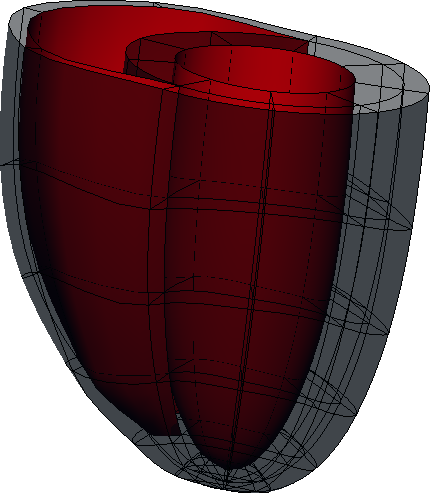
\includegraphics[width=.45\linewidth]{gfx/sham_mesh.png}}\quad
%     \subfloat[aortic-banded rat mesh.]
%     {\label{fig:ratrepmesh-b}
%     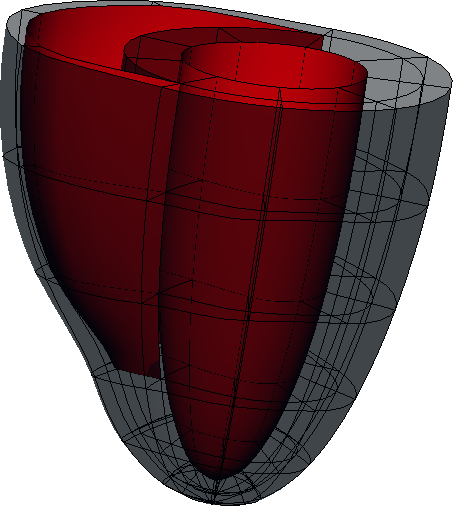
\includegraphics[width=.45\linewidth]{gfx/ab_mesh.png}}
%     \caption{Rat representative cubic Hermite finite element meshes.}\label{fig:ratrepmesh}
% \end{figure}

% \vspace{0.5cm}
% To mimic human pathological conditions, animal models are often established through life style, genetic or surgical procedures. In particular, left ventricular (LV) hypertrophy and compromised diastolic function can be caused by pressure overload, induced in rats by surgically constricting the aorta to impede blood flow. The constriction can be performed at different locations: transverse aorta, ascending aorta (shown in Figure~\ref{fig:aortic_banding}) or abdominal aorta, all causing an increase in aortic resistance and in LV end-diastolic pressure \cite{ku2016}. Cardiac hypertrophy and remodelling can be observed several weeks after the aortic constriction surgery. Since aortic constriction (especially in the abdominal aorta) requires simple experimental, surgical techniques \cite{ku2016}, aortic-banded (AB) rats are commonly used as an experimental animal model for HFpEF pathology \cite{patten2009, houser2012, conceicao2016, camacho2016}.

% % \begin{figure}[H]
% %     \centering
% %     \includegraphics[width=0.5\textwidth]{figures/aortic_banding_wiki.png}
% %     \caption{Aortic anatomy and one possible location for the banding (ascending aorta). Credit: Wikipedia.}
% %     \label{fig:aortic_banding}
% % \end{figure}

% \vspace{0.5cm}
% In the Introduction, we firstly introduce cardiac physiology. In that context, we will understand the importance of $\Ca$ ion, which represents the interface between the electrophysiological system and the mechanical system. We then provide a review of cardiac modelling, before summarising the work to date on simulating the rat heart.


